%chapter 7
\chapter{Environmental Effects of Transportation, Fuel Consumption Models and Emission Standards}
\section{Introduction}
Transportation activities, both passenger and freight, is crucial to economic activity, as it allows an increase in the flow of people and goods globally. Investment in transportation is fundamental for economic growth and development; the movement of people and goods from one place to another enables the exchange of goods and manpower, stimulating trade and commerce, and thus economic development. However, transport comes at a price having undesirable environmental impacts, which are generally referred to as \textit{externalities}.\\\\
As the environmental impacts of transportation increase with the flow
of transportation demand, the need to mitigate these is paramount. There are often several objectives that transportation strives to meet, which relate to economic, social and environmental aspects. However, it is not always possible to meet all the objectives simultaneously, which sometimes results in a compromise in one or more of the objectives, depending on the trade-offs.\\\\
This chapter discusses about the various externalities resulted due to extensive transportation activities. Most of these externalities are resulted due to vehicular emissions, therefore we will discuss about the fuel consumption models to quantify the fuel consumption contributed by vehicles. Lastly, this chapter also discusses about the various emission standards incorporated globally.
%
\section{Environmental Problems due to Transportation}
\subsection{Vehicular Emissions and Air Pollution}
Being arguably the most prominent of externalities, emissions are a consequence of use of fuel within the transport sector, such as liquid fuel, most of which is produced from petroleum. Gasoline and diesel are two of the most widely used types of liquid fuels, both of which are composed of many different types of hydrogen and carbon compounds, known as hydrocarbons, in which hydrogen and carbon atoms are chemically bound. Hydrocarbons include, for example, methane ($ CH_4 $) and ethane ($ C_2H_6 $).\\\\
Engines used in a majority of transportation vehicles, and particularly in
road transport, produce energy by mixing hydrocarbons with air. Volumewise, a large fraction of air contains oxygen ($ O_2 $) and nitrogen ($ N_2 $). The process by which energy is produced by engines is known as internal combustion, which, under ideal conditions, should only result in carbon dioxide ($ CO_2 $) and water vapour ($ H_2O $). However, the process is incomplete, meaning that not all of the fuel is consumed during internal combustion. As a result, a number of by-products are generated, such as carbon monoxide ($ CO $) as a result of insufficient oxygen, nitrogen oxide ($ NO_x $) as a result of nitrogen reacting with oxygen and particulate matter (PM) which are small particles of dust, soot and organic matter suspended in the atmosphere. In addition, small amounts of methane ($ CH_4 $) and nitrous oxide ($ N_2O $) are also produced during the combustion process. Furthermore, when sunlight reacts with air that contains hydrocarbons and NOx, it produces another gas called ozone ($ O_3 $). In maritime transportation, ships running on diesel engines burn fuel that contains high amounts of sulphur content, as a result of which sulphur oxide as well as nitrogen oxide emissions (also known as $ NO_x $ and $ SO_x $) are significant. The existence of these gases in the atmosphere gives rise to air pollution.\\\\
Some of the environmental impacts of vehicular emissions and air pollution are
discussed below.
\subsubsection{Particulate Matter (PM)}
Particulate matter is the general term for the mixture of solid particles and liquid droplets found in the air. Particulate matter includes dust, dirt, soot, smoke and liquid droplets. It can be emitted into the air from natural and man made sources, such as windblown dust, motor vehicles, construction factories, and fires. Particles are also formed in the atmosphere by condensation or the transformation of emitted gases such as sulphur dioxide, nitrogen oxides, and volatile organic compounds. sites, factories, and fires. Particles are also formed in the atmosphere by condensation or the transformation of emitted gases such as sulphur dioxide, nitrogen oxides, and volatile organic compounds.\\\\
Scientific studies show a link between particulate matter (alone or in combination with other
pollutants in the air) and a series of health effects. Studies of human populations and laboratory studies of animals and humans have established linkages to major human health impacts including respiratory symptoms; aggravation of existing respiratory and cardiovascular disease; alterations in the body’s defence systems against foreign materials; damage to lung tissue; carcinogenesis, and premature mortality.\\\\
PM also causes damage to materials and soiling; it is a major cause of substantial visibility impairment in many parts of the world.\\\\
Motor vehicle particle emissions and the particles formed by the transformation of motor vehicle gaseous emissions tend to be in the fine particle range. Fine particles (those less than 2.5 micrometers in diameter) are of health concern because they easily reach the deepest recesses of the lungs. Scientific studies have linked fine particles (alone or in combination with other air pollutants), with a series of significant health problems, including premature death; respiratory related hospital admissions and emergency room visits; aggravated asthma; acute respiratory symptoms, including aggravated coughing and difficult or painful breathing; chronic bronchitis; and decreased lung function that can be experienced as shortness of breath.\\\\
The US Environment Protection Agency (EPA) recently tightened the air quality standards for particulates. The standard for coarse particles (10 microns or less) remains essentially unchanged, while a new standard for fine particles (2.5 microns or less) was set at an annual limit of 15 micrograms per cubic meter and a 24-hour limit of 65 micrograms per cubic meter.\\\\
The California Air Resources Board (CARB) has evaluated diesel exhaust as a candidate toxic air
contaminant under the State's air toxics identification programme. To evaluate whether or not diesel exhaust causes cancer, the Office of Environmental Health Hazard Assessment (OEHHA) reviewed all controlled animal and mutagenicity studies as well as studies of worker populations exposed to diesel exhaust. They analysed over 30 human studies concerning lung cancer risk and workplace exposure to diesel exhaust. They found that workers who were exposed to diesel exhaust were consistently more likely than others to develop lung cancer. The consistent results are unlikely to be due to chance, confounding, or bias, according to CARB.\\\\
As a result, CARB concluded that a reasonable and likely explanation for the increased rates of lung cancer observed in the epidemiological studies is a causal association between diesel exhaust exposure and lung cancer.
%
\subsubsection{Carbon Monoxide ($ CO $)}
Carbon monoxide (CO) is a tasteless, odourless, and colourless gas produced though the incomplete combustion of carbon-based fuels. CO enters the bloodstream through the lungs and reduces the delivery of oxygen to the body’s organs and tissues. The health threat from exposure to low concentrations of CO is most serious for those who suffer from cardiovascular disease, particularly those with angina or peripheral vascular disease. Healthy individuals also are affected, but only at higher exposure levels. Exposure to elevated CO levels is associated with impairment of visual perception, work capacity, manual dexterity, learning ability and performance of complex tasks.
\subsubsection{Nitrogen Oxides ($ NO_x $)}
$ NO_x $ emissions produce a wide variety of health and welfare effects. Nitrogen dioxide can irritate the lungs and lower resistance to respiratory infection (such as influenza). $ NO_x $ emissions are an important precursor to acid rain that may affect both terrestrial and aquatic ecosystems. Atmospheric deposition of nitrogen leads to excess nutrient enrichment problems (“eutrophication”) a problem, for example, in the Chesapeake Bay and several other nationally important estuaries along the East and Gulf Coasts of the USA. Eutrophication can produce multiple adverse effects on water quality and the aquatic environment, including increased nuisance and toxic algal blooms, excessive phytoplankton growth, low or no dissolved oxygen in bottom waters, and reduced sunlight causing losses in submerged aquatic vegetation critical for healthy estuarine ecosystems. Nitrogen dioxide and airborne nitrate also contribute to pollutant haze, which impairs visibility and can reduce residential property values and revenues from tourism.
\subsubsection{Photo-chemical Oxidants (Ozone)}
Ozone is not emitted directly into the atmosphere, but is formed by a reaction of volatile organic compounds (VOC) — for vehicles mainly hydrocarbons (HC) — and $ NO_x $ in the presence of heat and sunlight. Ground-level ozone forms readily in the atmosphere, usually during hot summer weather. VOCs are emitted from a variety of sources, including motor vehicles, chemical plants, refineries, factories, consumer and commercial products, and other industrial sources. VOCs are also emitted by natural sources such as vegetation. $ NO_x $ is emitted from motor vehicles, power plants and other source of combustion. Changing weather patterns contribute to yearly differences in ozone concentrations and differences from city to city. Ozone can also be transported into an area from pollution sources found hundreds of miles upwind.\\\\
Ground-level ozone is the prime ingredient of smog, the pollution that blankets many areas during the summer4. Short-term exposures (1-3 hours) to high ambient ozone concentrations have been linked to increased hospital admissions and emergency room visits for respiratory problems. Repeated exposures to ozone can exacerbate symptoms and the frequency of episodes for people with respiratory diseases such as asthma. Other health effects attributed to short-term exposures include significant decreases in lung function and increased respiratory symptoms such as chest pain and cough. These effects are generally associated with moderate or heavy exercise or exertion. Those most at risk include children who are active outdoors during the summer, outdoor workers, and people with pre-existing respiratory diseases like asthma. In addition, long-term exposures to ozone may cause irreversible changes in the lungs, which can lead to chronic ageing of the lungs or chronic respiratory disease.\\\\
Ambient ozone also affects crop yield, forest growth, and the durability of materials. Because ground-level ozone interferes with the ability of a plant to produce and store food, plants become more susceptible to disease, insect
attack, harsh weather and other environmental stresses. Ozone
chemically attacks elastomers (natural rubber and certain synthetic polymers), textile fibres and dyes, and, to a lesser extent, paints. For example, elastomers become brittle and crack, and dyes fade after exposure to ozone.\\\\
Ozone is also an effective greenhouse gas, both in the stratosphere and the troposphere5. That is, ozone absorbs infrared radiation emitting from the earth, captures it before it escapes into space, and re-emits a portion of it back toward the earth’s surface. The specific role of ozone in climate change is very complex and not yet well understood. Ozone concentrations in the atmosphere vary spatially, both regionally and vertically, and are most significant in urban areas where precursor gases are abundant. This variability makes assessment of global, long-term trends difficult.
\subsubsection{Lead}
Over the past century, a range of clinical, epidemiological and toxicological studies have defined the nature of lead toxicity and investigated its mechanisms of action, identifying young children as a critically susceptible population. As noted by the 1995 Environmental Health Criteria Document for Lead, published by the International Programme on Chemical Safety (IPCS), lead affects many organs and organ systems in the human body with sub-cellular changes and neuro-developmental effects appearing to be the most sensitive. The most substantial evidence from cross sectional and prospective studies of populations with lead levels generally below 25 µg/decilitre of blood relates to reductions in intelligence quotient (IQ).\\\\
As noted by the IPCS, existing epidemiological studies do not provide definitive evidence of a threshold. Below the range of about 10-15 µg /decilitre of blood, the effects of confounding variables and limits in the precision in analytical and psychometric measurements increase the uncertainty attached to any estimate of effect. However, there is some evidence of an association below this range. Animal studies provide support for a causal relationship between lead and nervous system effects, reporting deficits in cognitive functions at lead levels as low as 11-15 µg/decilitre of blood which can persist well beyond the termination of lead exposure. Other effects, which may occur, include:
\begin{itemize}
	\item impaired sensory motor function;
	\item impaired renal function;
	\item a small increase in blood pressure has been associated with lead exposure;
	\item some but not all epidemiological studies show a dose dependent association of pre-term delivery and some indices of foetal growth and maturation at of 15 µg/decilitre or more.
\end{itemize}
Lead and its compounds may enter the environment at any point during mining, smelting, processing, use, recycling or disposal. In countries where leaded gasoline is still used, the major air emission is from mobile and stationary combustion of gasoline. Areas in the vicinity of lead mines and smelters are subject to high levels of air emissions.\\\\
Airborne lead can be deposited on soil and water, thus reaching humans through the food chain and in drinking water. Atmospheric lead is also a major source of lead in household dust.\\\\
Because of the concerns highlighted above, a global consensus has emerged to phase out the use of lead in gasoline.\\\\
In December 1994, at the Summit of the Americas, heads of state from a number of countries pledged to develop national action plans for the phase out of leaded gasoline in the Western Hemisphere.\\\\
In May 1996, the World Bank called for a global phase out of leaded gasoline and offered to help countries design feasible phase out schedules and incentive frameworks.\\\\
A key recommendation of the Third “Environment for Europe” Ministerial Conference held in Sofia, Bulgaria in October 1995 called for the reduction and ultimate phase out of lead in gasoline.\\\\
In June 1996, the second United Nations Conference on Human Settlements, called Habitat II, included the elimination of lead from gasoline as a goal in its agenda.\\\\
In May 1997, environmental ministers from the Group of Seven plus Russia endorsed the phase out of leaded gasoline in the 1997 Declaration of Environmental Leaders of the Eight on Children’s Environmental Health.
\subsubsection{Climate Change}
Beyond direct adverse health effects, there are other concerns with vehicle emissions. Among these is global warming or the greenhouse effect. Greenhouse warming occurs when certain gases allow sunlight to penetrate to the earth but partially trap the planet's radiated infrared heat in the atmosphere. Some such warming is natural and necessary. If there were no water vapour, carbon dioxide, methane, and other infrared absorbing (greenhouse) gases in the atmosphere trapping the earth's radiant heat, our planet would be about 60°F (33°C) colder, and life as we know it would not be possible. Naturally occurring greenhouse gases include water vapour, carbon dioxide ($ CO_2 $), methane ($ CH_4 $), nitrous oxide ($ N_2O $), and ozone ($ O_3 $).\\\\
Several classes of halogenated substances that contain fluorine, chlorine, or bromine are also greenhouse gases, but they are, for the most part,
solely a product of industrial activities. Chlorofluorocarbons (CFCs) and hydrochlorofluorocarbons (HCFCs) are halocarbons that contain chlorine, while halocarbons that contain bromine are referred to as halons. Other fluorine containing halogenated substances include hydrofluorocarbons (HFCs), perfluorocarbons (PFCs), and sulphur hexafluoride ($ SF_6 $).\\\\
There are also several gases that, although they do not have a direct global warming effect, do influence the formation and destruction of ozone, which does have such a terrestrial radiation absorbing effect. These gases include carbon monoxide (CO), oxides of nitrogen ($ NO_X $), and non-methane volatile organic compounds (NMVOCs).\\\\
Aerosols, extremely small particles or liquid droplets often produced by emissions of sulphur dioxide ($ SO_2 $), can also affect the absorptive characteristics of the atmosphere.\\\\
Although CO2, CH4, and N2O occur naturally in the atmosphere, the atmospheric concentration of
each of them has risen, largely as a result of human activities. Since 1800, atmospheric concentrations of these greenhouse gases have increased by 30, 145, and 15\%, respectively (IPCC 1996). This build-up has altered the composition of the earth’s atmosphere, and may affect the global climate system.\\\\
Beginning in the 1950s, the use of CFCs and other ozone depleting substances (ODSs) increased
by nearly 10\% a year, until the mid-1980s when international concern about ozone depletion led to the signing of the Montreal Protocol. Since then, the consumption of ODSs has rapidly declined, as they are phased-out.
In contrast, use of ODS substitutes such as HFCs, PFCs, and $ SF_6 $ has grown
significantly and all have strong greenhouse forcing effects.
\subsection{Noise Pollution}
Transport gives rise to noise pollution, primarily in urban areas, with undesirable effects on human health. These effects can range from short-term annoyance, sleep disturbance and impaired cognitive functioning to significant long-term physiological problems such as cardiovascular diseases, loss of hearing and mental health problems.
\subsection{Land and resource consumption}
Natural resources are depleted for use in the form of fuel, as well as by extraction of the materials required for building or construction. In addition, the infrastructure itself necessary for transportation activities (roads or highways, railway tracks, ports or terminals, storage or distribution facilities) damages land and local ecosystems.
%
\section{Mitigating measures}
Various approaches have been suggested to reduce the environmental impacts of transportation, some of which are described here:
\begin{itemize}
	\item \textbf{\textit{Technological improvements}} are aimed at developing new technology to improve the environmental performance of vehicles, including improved design of vehicles that allow for additional carrying capacity without compromising the fuel or energy efficiency, new vehicles that run on alternative sources of energy (such as electric vehicles or alternative fuels such as bio-diesel) and new design or redesign of engines that have better energy efficiency.
	\item \textbf{\textit{Strategic or tactical approaches}} include changing the so-called modal split of freight and transferring freight from energy-intensive modes of transport, such as road, to more environmentally friendly modes of transport, for example rail, coastal shipping, waterways, or use of any of these in combination with road transport. Tactical approaches also include fleet management involving the selection of the right vehicles to purchase and maintain, as well as regular vehicle maintenance to ensure that they operate at optimum efficiency. In road transportation, for example underinflated tires, fuel leaks or poor combustion can lead to loss in fuel efficiency of a vehicle.
	\item \textbf{\textit{Operational strategies}} include reducing the actual numbers of vehicles running, vehicle kilometers and tonne kilometers by increasing load factors (reducing empty or partly loaded running of lorries), utilizing new information technology to improving the routing and scheduling of vehicles, consolidating deliveries, sharing loads and pick up deliveries with other companies and improving driver training and behavior.
\end{itemize}
It is important that these approaches are implemented to produce win-win solutions, in which the environmental benefits should be at least as much as the gains reaped by the organizations or companies who adopt these practices.
\subsubsection{Kyoto Protocol}
In late November 1995, the IPCC Working Group 1 concluded, “the balance of evidence suggests that there is a discernible human influence on global climate.” In December 1997, acting on this consensus, countries around the world approved the Kyoto Protocol to the 1992 Climate Change Treaty. Key aspects of the agreement include:
\begin{description}
	\item [Reductions:] Thirty-eight industrialized nations are required to reduce their “greenhouse” gas emissions from 1990 levels between 2008 and 2012. The European Union would reduce them by 8\%, the United States by 7\% and Japan by 6\%. Some would face smaller reductions, and a few would not face any now. As a group, the industrialized nations would cut back on the emissions of such gases by just more than 5\%.
	\item [Gases Involved:] Emissions of six gases would be affected: carbon dioxide, methane, nitrous oxide, and three halo-carbons used as substitutes for ozone-damaging chlorofluorocarbons.
	\item ['Offshore' Reductions:] Countries that do not meet their own emission targets can strike deals with nations that do better than required, to buy the excess “quota”. This may encourage reductions to be made where most cost-effective.
	\item [Enforecement:] A later meeting of the treaty parties will decide on “appropriate and effective” ways to deal with non-compliance.
	\item [Developing Countries:] Developing countries, including major greenhouse gas emitters such as China and India, are asked to set voluntary reduction targets.
	\item [Next Step:] The accord approved by the Kyoto conference takes effect once it is ratified by 55 nations, representing 55\% of 1990 carbon dioxide emissions. It is binding on individual countries only after their governments' complete ratification.
\end{description}
Implementing this agreement requires significant improvements in fuel economy and carbon dioxide emissions from vehicles.
%
\section{Fuel Consumption Models}
Fuel consumption models are mathematical relationships giving fuel consumption as a function a function of other measurable or calculable quantities that are usually aggregated over the portion of the transportation system being analyzed. The quantities measured or calculated may be vehicle-miles traveled, number of stops per unit of time, total vehicular delay per unit of time, average speed, and so on. Two forms that have found the most use in practice to date are drive-mode elemental models and average-speed models.
\subsection{Drive-Mode Elemental Models}
As the name implies, drive-mode elemental models are made up of the elements that contribute to fuel consumption while driving (i.e., fuel used in cruising, idling, and accelerating). The basic assumptions in an elemental model are that the elements are independent and their sum equals the total fuel consumed.\\\\
The simplest form of drive-mode elemental model is:
\begin{equation}
	G = f_1 L + f_2 D + f_3 S
\end{equation}
Where,\\
\hspace*{10mm} $ G $ = fuel consumed per vehicle over a measured distance (total section distance)\\
\hspace*{10mm} $ L $ = total section distance traveled\\
\hspace*{10mm} $ D $ = stopped delay per vehicle (i.e., time spent in idling)\\
\hspace*{10mm} $ S $ = number of stops\\
\hspace*{10mm} $ f_1 $ = fuel consumption rate per unit distance traveled while cruising\\
\hspace*{10mm} $ f_2 $ = fuel consumption rate per unit time while idling\\
\hspace*{10mm} $ f_3 $ = excess fuel used in decelerating to stop and accelerating back to cruise speed
%
\subsection{Average-Speed Models}
The model relating fuel consumption to trip time or its inverse, average speed is:
\begin{equation}
	F = k_1 + k_2 T = k_1 + \frac{k_2}{v}
\end{equation}
$$ for\: 10 \leq v \leq 56\:kmph $$
Where,\\
\hspace*{10mm} $ F $ = fuel consumed per vehicle per unit distance (e.g., liters/km or gal/mi)\\
\hspace*{10mm} $ T $ = travel time per unit distance, including stops and speed changes (e.g., min/km or min/mi)\\
\hspace*{10mm} $ v $ = average speed measured over a distance, including stops and speed changes\\
\hspace*{10mm} $ k_1 $ = parameter associated with fuel consumed to overcome rolling resistance, approximately proportional to vehicle weight (gal/veh-mi)\\
\hspace*{10mm} $ k_2 $ = parameter approximately proportional to fuel consumption while idling (gal/hr)\\\\
This form of the average speed model is not valid at speeds higher than 56 km/hr (35 mph) because at higher speeds the effects of air resistance become increasingly stronger. For speeds lower than 15 km/hr (9 mph), fuel consumption increases rapidly and a better fit to the data is:
\begin{equation}
	F = F_R + \frac{800 F_0}{v (v + 8)}
\end{equation}
Where,\\\\
\hspace*{10mm} $ F_R $ = fuel consumed while in motion (liters/100 km)\\
\hspace*{10mm} $ F_0) $ = fuel consumed during stopped time while idling (liters/hr)\\
\hspace*{10mm} $ v $ = average speed (km/hr)\\\\
The validity of the average-speed model have been estimated from regression analysis of fuel consumption data in several countries. Data on 37 U.S. passenger cars on 1976 model year were found to be closely correlated with vehicle weight and fuel rate at idle, giving the relationships:
\begin{gather}
	\because k_1 = 9.5\times 10^{-6} \: W \: (gal/mi)\\
	\: \: = 49.57 \times 10^{-6} Wm \: (liter/km)\\
	\because k_2 = 0.998 I = I \times f_2
\end{gather}
Where,\\
\hspace*{10mm} $ W $ = vehicle weight (lb)\\
\hspace*{10mm} $ Wm $ = vehicle weight (kg)\\
\hspace*{10mm} $ I $ = fuel consumption rate while idling\\\\
Depending on vehicle weight, engine size, and technological features, the -values of $ k_1 $ and $ k_2 $ can vary widely. Data from field tests (1973-1976) on nine passenger cars ranging in weight from 2270 to 5474 lb (1035 to 2488 kg) gave values of $ k_1 $ ranging from 0.0194 to 0.0518 gal/mi (0.0456 to 0.1218 liter/km) and values of $ k_2 $ ranging from 0.418 to 1.031 gal/hr (For use in metric version of the model this would be equivalent to $ k_2 $ ranging from 0.983 to 2.42 in order to yield 1/km). The average values were incorporated into a version of model published by FHWA:
\begin{equation}
	F = 0.0362 + \frac{0.746}{v} (gal/veh-mi)
\end{equation}
By using the relationship $ k_1 $ = 9.58 $ \times 10^{-6} \:W$, the value of $ k_1 $ = 0.0362 represents a vehicle weighing 3800 lb (1718 kg).\\\\
Buses operating in an urban environment may present a unique case because of their schedule of frequent stops. In this case, bus fuel consumption may be calculated by using graphs such as the graph given below calibrated with average number of stops per unit distance rather than average speed. The estimate for stops should include both the scheduled stops and the stops resulting from traffic congestion and traffic controls.
\begin{center}
	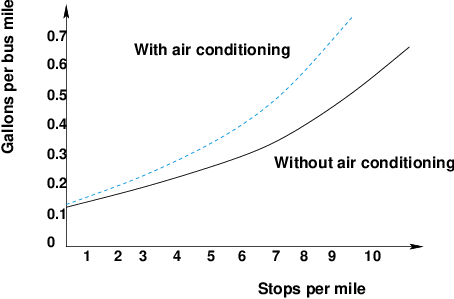
\includegraphics[scale=0.8]{gfx/fig55.png}
\end{center}
\section{Emissions Control Programmes}
\subsection{European Union}
The European Commission set up the European Auto-Oil Programme in 1994 with the European associations for the car industry (ACEA) and the oil industry (Europia), to provide the technical basis for the development of EU policy towards road vehicle emissions. The first phase of the programme was completed in 1996 and following two years of refinement, a three-part dossier to further reduce pollution from road transport in the Community was agreed, in 1998, by the European Parliament and the Council of Environment Ministers. The three dossiers cover:
\begin{itemize}
	\item measures to be taken against air pollution by emissions from passenger cars;
	\item measures to be taken against air pollution by emissions from light commercial vehicles (pick up trucks, delivery vans etc.);
	\item the quality of petrol and diesel fuels.
\end{itemize}
Overall the Auto Oil programme has five sections:
\begin{itemize}
	\item fuel quality;
	\item emissions from private cars;
	\item emissions from light commercial vehicles;
	\item emissions from heavy goods vehicles;
	\item adaptation of provisions relating to roadworthiness testing.
\end{itemize}
More specifically, the directives aim at:
\begin{itemize}
	\item Controlling those parameters in the composition of petrol and diesel that influence the level of atmospheric emissions, in particular sulphur, benzene, aromatics and lead;
	\item Reducing the limit values for certain pollutants in new vehicle models being brought onto the market;
	\item In addition, improved control of the day-to-day emissions of vehicles in use is to be achieved by the mandatory fitting of on-board diagnostic systems, the introduction of a new testing procedure and a new test to limit evaporative emissions.
\end{itemize}
EU has been regulating these standards gradually imposing more stringent standards to eventually reduce emissions. The following is a summary list of the standards, and when they come into force:
\begin{itemize}
	\item Euro 1 (1992)
	\item Euro 2 (1996)
	\item Euro 3 (2000)
	\item Euro 4 (2005)
	\item Euro 5 (2009)
	\item Euro 6 (2014)
\end{itemize}
\subsection{India}
Bharat stage emission standards (BSES) are emission standards instituted by the Government of India to regulate the output of air pollutants from internal combustion engines and Spark-ignition engines equipment, including motor vehicles. The standards and the timeline for implementation are set by the Central Pollution Control Board under the Ministry of Environment \& Forests and climate change. These standards, based on European regulations, were first introduced in 2000. n 2014, Saumitra Chaudhary committee gave recommendations on Auto Fuel Vision Policy 2025 which had recommended implementation of BS-IV (2017), BS-V (2019) and BS-VI (2024) standards. In 2016, the Indian government announced that the country would skip the BS-V norms altogether and adopt BS-VI norms by 2020. While the norms help in bringing down pollution levels, it invariably results in increased vehicle cost due to the improved technology \& higher fuel prices. Currently, BS IV norms have been enforced across the country since April 2017. However, recently the Supreme Court of India ordered barring of sale of Bharat Stage IV vehicles from April 1, 2020.
